\documentclass[a4paper, 12pt]{article}

\usepackage[english]{babel}
%\usepackage[portuges]{babel}
\usepackage[utf8]{inputenc}
\usepackage{amsmath}
\usepackage{indentfirst}
\usepackage{graphicx}
\usepackage{multicol,lipsum}
%\renewcommand{\figurename}{Figura}
\usepackage[hidelinks]{hyperref}
\usepackage{rotating}
\usepackage{lscape}

%%%%%%%%%%%%%%%%%%%%%%%%%%%%%%%%%%%
\usepackage{pythonhighlight}
%%%%%%%%%%%%%%%%%%%%%%%%%%%%%%%%%%%

\setlength{\parskip}{1em}

\begin{document}
%\maketitle

\begin{titlepage}
	\begin{center}
	
	%\begin{figure}[!ht]
	%\centering
	%\includegraphics[width=2cm]{c:/ufba.jpg}
	%\end{figure}

		\textbf{\Large{BRP Report}}\\
		\large{Data Quality Analyst Assignment}\\ 
		%\large{Programa}\\ 
		\vspace{15pt}
        \vspace{95pt}
        %\textbf{\large{Rascunho PEP}}\\
		%\title{{\large{Título}}}
		\vspace{3,5cm}
	\end{center}
	
	\begin{flushleft}
		\begin{tabbing}
			Kallil de Araujo Bezerra \\
	\end{tabbing}
 \end{flushleft}
	\vspace{1cm}
	
	\begin{center}
		\vspace{\fill}
			\today
	\end{center}
\end{titlepage}
%%%%%%%%%%%%%%%%%%%%%%%%%%%%%%%%%%%%%%%%%%%%%%%%%%%%%%%%%%%

% % % % % % % % %FOLHA DE ROSTO % % % % % % % % % %

% % % % % % % % % % % % % % % % % % % % % % % % % %
\newpage
\tableofcontents
\thispagestyle{empty}

\newpage
\pagenumbering{arabic}
% % % % % % % % % % % % % % % % % % % % % % % % % % %
\section{Task 1}

The goal of the first task is to present the data so we can familiarize ourselves with what's presenting.

\subsection{A - Read both .csv files into Python}
Reading both files using Python:

First, two variables were created. One for each file, and they carry the string that represents their location, so if we ever need to change the path it can be easily done by just changing the value stored by the variable.

\begin{python}
	dealer_data_path = "/content/sample_data/DEALER.csv"
	retail_data_path = "/content/sample_data/RETAIL_SALES.csv"
\end{python}

After that, we can load the files using:

\begin{python}
	df_dealer = pd.read_csv(dealer_data_path)
	df_retail = pd.read_csv(retail_data_path)
\end{python}

\subsection{B - Display the data types for each column for both datasets}

Again, we create variables to store their data types, and if we need to change something here it's possible to do it by just changing the values in the variables.

\begin{python}
	dealer_data_types = df_dealer.dtypes
	retail_data_types = df_retail.dtypes
\end{python}

\begin{python}
	print("1 B:\n")
	print("Data types for the dealer dataset:\n")
	print(dealer_data_types)
	
	print("\n----//----//----//----//----//----//----//----")
	print("\nData types for the retail dataset:\n")
	print(retail_data_types)
\end{python}

The result of this code (for the dealer dataset) can be seen in figure \ref{img_01}.

\begin{figure}[!htb]
	\caption{\label{img_01} Data types}
	\begin{center}
		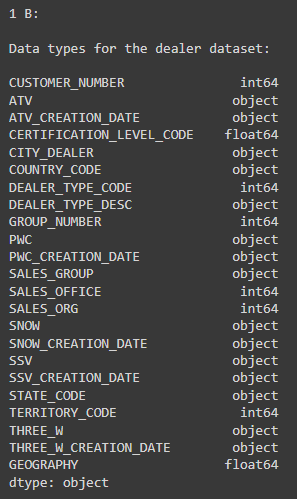
\includegraphics[scale=1.10]{img_01.PNG}
	\end{center}
\end{figure}

\subsection{C - What is the number of rows and columns for each dataset?}

Moving on, we need to see the size of our dataset. To do this we can use the \textit{shape} method from \textit{Pandas}.

\begin{python}
	dealer_data_rows = df_dealer.shape
	retail_data_rows = df_retail.shape
\end{python}

\begin{python}
	print("1 C:\n")
	print("Number of rows and columns in the dealer dataset")
	print("# of rows: {}".format(dealer_data_rows[0]))
	print("# of columns: {}\n".format(dealer_data_rows[1]))
	
	print("----//----//----//----//----//----//----//----")
	print("\nNumber of rows and columns in the retail dataset")
	print("# of rows: {}".format(retail_data_rows[0]))
	print("# of columns: {}".format(retail_data_rows[1]))
\end{python}

The results can be seen in figure \ref{img_02}.

\begin{figure}[!htb]
	\caption{\label{img_02} Data shape}
	\begin{center}
		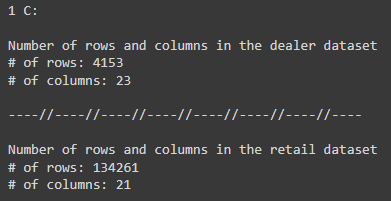
\includegraphics[scale=1.10]{img_02.PNG}
	\end{center}
\end{figure}

\subsection{D - Display the first 6 rows for the DEALER dataset and the last 8 for the RETAIL\_SALES one}

\begin{python}
	dealer_top_six = df_dealer.head(6)
	retail_bot_eight = df_retail.tail(8)
\end{python}

\begin{python}
	print("The first 6 rows in the dealer dataset are:")
	print(dealer_top_six)
	
	print("\n----//----//----//----//----//----//----//----")
	print("\nThe last 8 rows in the retail data set are:")
	print(retail_bot_eight)
\end{python}

The results can be seen in figures \ref{img_03a} and \ref{img_03b}, but they're not complete because the images would take too much space in the report.

\begin{figure}[!htb]
	\caption{\label{img_03a} First 6 rows of the DEALER dataset}
	\begin{center}
		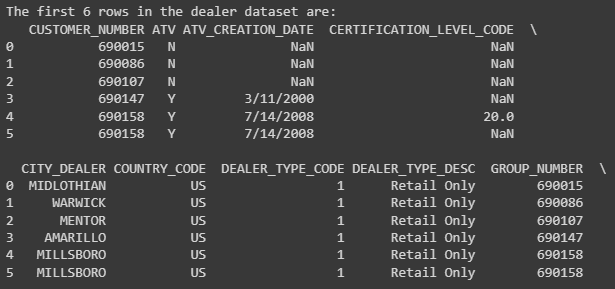
\includegraphics[scale=0.8]{img_03a.PNG}
	\end{center}
\end{figure}

\begin{figure}[!htb]
	\caption{\label{img_03b} Last 8 rows of the RETAIL dataset}
	\begin{center}
		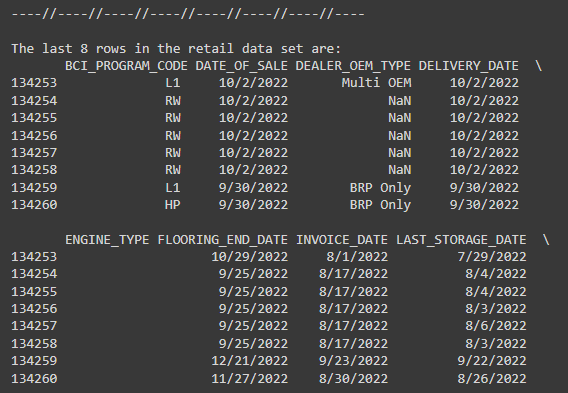
\includegraphics[scale=0.8]{img_03b.PNG}
	\end{center}
\end{figure}

\newpage
\section{Task 2}

Now that the dataset is better understood, we can proceed with some data cleaning.

\subsection{A - Remove duplicated lines in the DEALER dataset. How many of duplicated lines there were?}

There were 5 duplicate rows in the original dataset. Below is the code that was used to do this analysis.

\begin{python}
	df_duplicates_dropped = df_dealer.drop_duplicates(keep='first', inplace=False)
	num_duplicates_dropped = len(df_dealer) - len(df_duplicates_dropped)
\end{python}

\begin{python}
	print("Number of Duplicate Rows Dropped: {}" .format(num_duplicates_dropped))
\end{python}

\begin{figure}[!htb]
	\caption{\label{img_4} Dropping and counting how many duplicate rows the dataset had}
	\begin{center}
		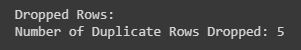
\includegraphics[scale=1.1]{img_04.PNG}
	\end{center}
\end{figure}

After that, I dropped and saved the new 

\subsection{B - How many NAs exist within the CITY\_DEALER column in the DEALER dataset? Replace the NA values for the string:  no city found.}

There were 3 occurrences of CITY\_DEALER with NA or empty values.

\begin{python}
	dealer_na_cities = df_dealer['CITY_DEALER'].isna().sum()
	print('There are {} occurrences of NA or empty cities'.format(dealer_na_cities))
\end{python}

\begin{figure}[!htb]
	\caption{\label{img_5} Total number of NA or empty CITY\_DEALER}
	\begin{center}
		
\includegraphics[scale=1.1]{img_05.PNG}
	\end{center}
\end{figure}

Now we swap those NA or empty values for \textit{no city found}.

\begin{python}
	df_dealer['CITY_DEALER'].fillna('no city found', inplace = True)
\end{python}

\subsection{C - Filter the DEALER dataset to include only dealers with COUNTRY\_CODE US or CA}

\begin{python}
	df_dealer = df_dealer[(df_dealer['COUNTRY_CODE'] == 'US')|(df_dealer['COUNTRY_CODE'] == 'CA')]
\end{python}

\subsection{D - In the RETAIL\_SALES dataset, remove the trailing x (xxx) of the column REG\_DEALER\_NUMBER}

\begin{python}
	df_retail['REG_DEALER_NUMBER'] = df_retail['REG_DEALER_NUMBER'].str.replace('x', '', regex=True)
\end{python}

\subsection{E - Keep only the following columns in the DEALER dataset: CUSTOMER\_NUMBER, CITY\_DEALER, COUNTRY\_CODE and STATE\_CODE}

\begin{python}
	df_dealer = df_dealer[['CUSTOMER_NUMBER', 'CITY_DEALER', 'COUNTRY_CODE', 'STATE_CODE']]
\end{python}

\section{Task 3}

\subsection{A - In the RETAIL\_SALES dataset, create a column named RETAIL and assign the integer 1 to it}

\begin{python}
	df_retail['RETAIL'] = 1
\end{python}

\subsection{B - Set the datatypes of columns CUSTOMER\_NUMBER and REG\_DEALER\_NUMBER to integer for the DEALER and RETAIL\_SALES datasets respectively}

\begin{python}
	df_dealer['CUSTOMER_NUMBER'] = df_dealer['CUSTOMER_NUMBER'].astype(int)
	df_retail['REG_DEALER_NUMBER'] = df_retail['REG_DEALER_NUMBER'].astype(int)
\end{python}

\subsection{C - In the DEALER dataset, create a column called REGION\_CODE based on the STATE\_CODE columns. Each region is specified as per the dictionary provided in the original doc}

\begin{python}
	region_mapping = {
		1: ["AB", "BC", "MB", "NB", "NF", 
			  "NS", "NT", "NU", "ON", "PE", 
			  "QC", "SK", "YT"],
		2: ["AL", "CT", "DE", "DC", "FL", 
			  "GA", "MA", "MD", "ME", "NC", 
			  "NH", "NJ", "NY", "PA", "PR", 
			  "RI", "SC", "VA", "VT", "WV"],
		3: ["AR", "IA", "IL", "IN", "KS", 
			  "KY", "LA", "MI", "MN", "MO", 
			  "MS", "ND", "NE", "OH", "SD", 
			  "TN", "WI"],
		4: ["AK", "AZ", "CA", "CO", "HI", 
			  "ID", "MT", "NM", "NV", "OK", 
			  "OR", "TX", "UT", "WA", "WY"]
	}
	
	df_dealer['REGION_CODE'] = df_dealer['STATE_CODE'].apply(
	lambda state: next((region for region, states in region_mapping.items() if state in states), 5)
	)
\end{python}

\section{Task 4}

\subsection{A - Merge the DEALER dataset into the RETAIL\_SALES using CUSTOMER\_NUMBER and REG\_DEALER\_NUMBER columns. Explain why you selected this specific join type}

Before continuing, it's important to say that MODEL\_CODE does not exist, so I used MODEL\_NUMBER instead.

For this task I assumed that this data would be used for some kind of reporting, so we won't use the NA rows that would come up if we did an outer, left, or right join.

Therefore, the best option was a inner join, in which we will keep only the matching rows from both datasets.

\begin{python}
	df_merged_data = pd.merge(df_retail, df_dealer, left_on = 'REG_DEALER_NUMBER', right_on = 'CUSTOMER_NUMBER', how = 'inner')
\end{python}

\subsection{B - I - What is the overall top selling MODEL\_CODE in the STATE\_CODE of AZ and MB? Use the RETAIL column to calculate sales.}

\begin{python}
	top_selling_overall = df_merged_data[df_merged_data['STATE_CODE'].isin(['AZ','MB'])].groupby('MODEL_NUMBER')['RETAIL'].sum().idxmax()
\end{python}

This code will return a value, which is shown in figure \ref{img_7}.

\begin{figure}[!htb]
	\caption{\label{img_7} Most sold product in states AZ and MB}
	\begin{center}
		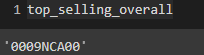
\includegraphics[scale=1.1]{img_07.PNG}
	\end{center}
\end{figure}

\subsection{B - II - What are the top 10 MODEL\_CODEs sold in REGION\_CODE number 3, in the year 2021? Use REGISTRATION\_DATE to calculate the dates}

\begin{python}
	df_merged_data['REGISTRATION_DATE'] = pd.to_datetime(df_merged_data['REGISTRATION_DATE'], format='%m/%d/%Y')
	df_merged_data['REG_YEAR'] = df_merged_data['REGISTRATION_DATE'].dt.year
\end{python}

\begin{python}
	filtered_data = df_merged_data[(df_merged_data['REGION_CODE'] == 3) & (df_merged_data['REG_YEAR'] == 2021)]
\end{python}

\begin{python}
	model_sales = filtered_data.groupby('MODEL_NUMBER')['RETAIL'].sum()
\end{python}

\begin{python}
	top_10_models_2021 = model_sales.nlargest(10)
	print(top_10_models_2021)
\end{python}

\begin{figure}[!htb]
	\caption{\label{img_6} Top 10 most sold products}
	\begin{center}
		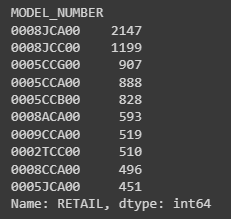
\includegraphics[scale=1.1]{img_06.PNG}
	\end{center}
\end{figure}

Therefore, the most sold product is the 008JCA00, with 2147 units sold. This can be verified in figure \ref{img_6}.

\newpage

\subsection{B - III - Create a chart to display the total sales per REGION\_CODE and year}

\begin{python}
	import matplotlib.pyplot as plt
	
	# Group the data by REGION_CODE and REG_YEAR and calculate the total sales
	total_sales_per_region_year = df_merged_data.groupby(['REGION_CODE', 'REG_YEAR'])['RETAIL'].sum()
	
	# Reset the index to make REGION_CODE and REG_YEAR columns accessible for plotting
	total_sales_per_region_year = total_sales_per_region_year.reset_index()
	
	# Create a pivot table to reshape the data for plotting
	pivot_table = total_sales_per_region_year.pivot(index='REG_YEAR', columns='REGION_CODE', values='RETAIL')
	
	# Plot the data as a bar chart
	ax = pivot_table.plot(kind='bar', stacked=False, figsize=(12, 6))
	plt.xlabel('Year')
	plt.ylabel('Total Sales')
	plt.title('Total Sales per REGION_CODE and Year')
	plt.legend(title='REGION_CODE', loc='upper right', bbox_to_anchor=(1.2, 1))
	
	for p in ax.patches:
	ax.annotate(str(int(p.get_height())), (p.get_x() + p.get_width() / 2., p.get_height()), ha='center', va='bottom')
	
	plt.show()
\end{python}

\begin{figure}[!htb]
	\caption{\label{img_8} Bar chart with sales per region and year}
	\begin{center}
		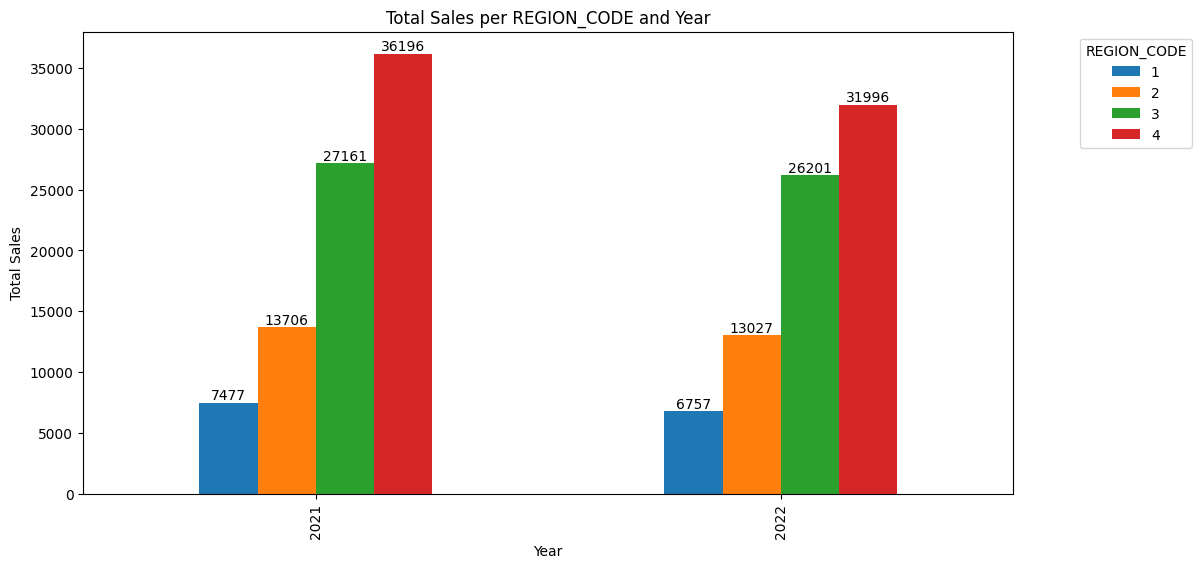
\includegraphics[scale=0.5]{img_08.PNG}
	\end{center}
\end{figure}



\newpage
\section{Task 5}

\subsection{A - Define at least 5 quality checks you would perform in the dataset with a brief explanation of their objective.}

\begin{enumerate}
	\item Date Standardization: Ensure consistent date formats by converting all date entries to a standardized format (e.g., YYYY-MM-DD). This standardization prevents format-related issues when processing the data.
	
	\item Special Character Cleanup: Remove special characters from data entries to maintain consistency when transferring data across different systems, such as from a Microsoft Server to Power BI or a CSV file.
	
	\item Data Validation and Standardization: Perform data validation to verify the accuracy and consistency of location-related data. Ensure that cities and state codes are valid, adhere to standard naming conventions, and eliminate duplicated or similar but distinct entries (e.g., 'Alexandria Bay' and 'Alexandria Bay,') to avoid data duplication.
	
	\item Duplicate Record Detection: Detect and handle duplicated records, which can distort analysis and decision-making. This can involve identifying identical records or reconciling records representing the same entity with variations in data entry.
	
	\item Missing Value Assessment: Check critical columns for missing values. Columns such as 'REG\_DEALER\_NUMBER' and 'MODEL\_NUMBER' should be complete, as they are important identifiers. Address any null or empty values to maintain data integrity.
\end{enumerate}

\end{document}



